\clearpage
\section*{S6 Other settings of TCLUST-REG, further competitors, repeated runs, and the third part of the study}
\label{supp:r10}

This section holds the detail behind Sections~4.4 to~4.6 and~5 of the paper. Throughout,
ESF is the flagging procedure of Algorithm~1 of the paper, ``rw'' the reweighting rule of the
paper (the map of its Section~3 applied twice, $c=2.5$, a median absolute deviation per
group), and the recovery step is Algorithm~2 of the paper.

\subsection*{S6.1 Other settings of TCLUST-REG}

With three and four groups the level $0.40$ loses part of a group. With equal group weights in
the assignment (option \texttt{equalweights} of FSDA), the long search, reweighting and the
recovery step, run on every data set, TCLUST-REG at this level reached $0.87$ in D2 and $0.86$
with four groups up to $\varepsilon=0.20$, against $0.83$ and $0.81$ with estimated weights,
and at level $0.25$ it reached $0.90$ and $0.96$ (ESF: $0.89$ and $0.95$). Part of the loss
thus comes from the estimated weights. Over all cells, equal weights changed the level $0.40$
little and made the level $0.25$ the most accurate pipeline up to $20\%$ of outliers, but not
beyond (Table~2 of the paper; Table~S39). With equal scales (restriction factor $1$; $300$
starts, D2 and the four-group design only) the level $0.40$ reached $0.86$ and $0.77$. Adaptive second-level trimming in the covariates (FSDA's option
$\alpha_X=0.99$, run with $300$ starts in D5 to D7 of the first two parts; the Octave run
needed one more one-line substitute, for \texttt{any(x,'all')}) did not help with
high-leverage points: at $\varepsilon=0.20$ it lowered the accuracy of TCLUST-REG with
reweighting and the recovery step from $0.83$ and $0.87$ to $0.80$ and $0.73$ at levels $0.25$
and $0.40$, and from $25\%$ of outliers it stayed at or below $0.63$; in D6 it moved the level $0.25$ by
$-0.025$ at $30\%$ and $+0.031$ at $35\%$,
and in D7 it lowered the level $0.40$ at $35\%$ from $0.90$ to $0.86$. FSDA's option
$\alpha_X=1$, which fits the cluster-weighted model, was not run; the trimmed cluster-weighted
model of RobMixReg represents that model in the study. Nor did the monitoring path give a
TCLUST-REG without a level. We fitted it at the levels $0,0.05,\dots,0.40$ ($300$ starts) and
compared consecutive classifications by the adjusted Rand index. Taking the first level at
which two consecutive classifications agree (index at least $0.9$) chose a level below the
contamination (a median of $0.05$ to $0.15$ for $\varepsilon\ge0.10$), and with reweighting and
the recovery step fell below $0.85$ in $36$ of the $89$ cells with $\varepsilon\le0.20$; taking
the smallest level from which all later consecutive classifications agree nearly always chose
$0.40$ and behaved like that level ($7$ cells below $0.85$, the worst $0.76$ with four groups).

\subsection*{S6.2 Further competitors and checks}

The following analyses were decided after the plans and run on every data set, and are
descriptive (Table~S39). The mixture of $t$ regressions of \citet{yao2014robust}, with a common
number of degrees of freedom and $20$ starts, fails like the other mixtures with three and four
groups ($0.38$ and $0.51$ up to $\varepsilon=0.20$) and with clustered outliers ($0.54$).
Robust linear grouping \citep{garciaescudero2009robust}, which draws random subsamples as ESF
does but fits orthogonal hyperplanes at a fixed level, often returned a nearly vertical
hyperplane: at level $0.25$ with reweighting and the recovery step its accuracy fell below
$0.85$ in $24$ of the $89$ cells with $\varepsilon\le0.20$. The incremental reweighting of
\citet{dotto2018reweighting}, which lowers the trimming level from $0.40$ to $0$ in steps of
$0.02$ and refits at each step, did not do better than the single reweighting step after
TCLUST-REG at level $0.40$: it recovered part of the small groups ($0.57$--$0.98$ against
$0.56$--$0.73$ up to $\varepsilon=0.20$), gained up to $0.03$ with three and four groups without
outliers and lost up to $0.13$ with them at $\varepsilon=0.20$, and fell below $0.85$ in $32$
cells, and in $22$ after the recovery step against four. Two changes to our own constants were
also tried. Taking the noise range of the recovery step over the unflagged units only, so that
the outliers do not set it, lost small groups (down to $0.62$ with groups of $85\%$ and $15\%$
at $\varepsilon=0.20$) and did not prevent the harm with uniform noise described in
Section~4.6 of the paper. Taking the scale of the scoring loss of ESF as the $10\%$ quantile of
the replicates' median squared residuals instead of their minimum, on parts one and three,
lowered the accuracy by up to $0.05$ with high-leverage points and uniform noise at
$\varepsilon=0.20$, and did not remove the loss with $B=500$.

\subsection*{S6.3 The comparison of Plan~1, the loss cap, repeated runs and the best-of-five rule}

The comparison of Plan~1 used the seven designs without high-leverage points and the four
levels $\varepsilon\le0.20$, $28$ cells, and no cell failed: the largest shortfall of ESF
alone against the best competitor was $0.029$ (standard error $0.014$), in D3 at
$\varepsilon=0.20$, and in $23$ of the $28$ cells it was below $0.005$ (Table~S1); for ESF with the recovery step (Plan~3) it was $0.017$, in
D3 at $\varepsilon=0.20$ ($0.016$ in D6), with the long-search rows and the later competitors included, and
that of ESF alone then becomes $0.031$, against sequential RANSAC in D3 at
$\varepsilon=0.20$, of the order of the variation between random seeds. The second criterion
of Plan~1 failed for TCLUST-REG at level $0.25$ with reweighting, never more than $0.033$
below ESF alone (D2, $\varepsilon=0$; at most $0.012$ with the long search), so this
competitor was tested again, on new data, at higher contamination.


A larger loss cap is no cure for the small groups that ESF alone flags: with $c_b=5$ the small
groups are largely recovered, but the accuracy falls from $0.91$ to $0.82$ in D1 and from
$0.88$ to $0.74$ in D7 at $\varepsilon=0.35$, and from $0.90$ to $0.79$ in D2 and from $0.85$
to $0.72$ in D5 at $\varepsilon=0.20$ (Table~S13).


In five runs with different seeds on each data set of the study, the accuracies of ESF
differed by more than $0.05$ on $3.5\%$ of the data sets with up to $20\%$ of outliers and on
$13\%$ of all data sets, most of them where ESF breaks down. More replicates do not remove the
small-group failure of ESF alone: with $B=500$ the largest losses were with small groups at
$30\%$ of outliers (Table~S29), because a wider search finds the fits with two lines on the large
group more often, which the scoring criterion allows (Section~2.3 of the paper); with a small
group, the recovery step is a necessity, not an option.

\paragraph{A default for real data (Section~2.5 of the paper).} The study used $B=100$ and one seed per data set. On the
fishery data (Section~5.1 of the paper) the answer depended on the seed, and two remedies
were examined there. Keeping, among five seeds, the fit of highest likelihood under the model
of the recovery step returned the modal fit every time over twenty disjoint sets of seeds; on
the simulated data it raised cell means by more than $0.005$ in $27$ of $102$ cells and never
lowered one by more than $0.001$ up to $20\%$ of outliers, but beyond it lowered one cell,
three groups at $35\%$, by $0.096$ (Table~S24). More replicates also reduced the
dependence on the fishery data, where with $B=100$, $500$ and $1000$ the modal fit was returned
by $17$, $18$ and $19$ of $20$ seeds with $K=2$ and by $14$, $18$ and $19$ with $K=3$, but on
the simulated data $B=500$ moved cell means by $-0.07$ to $+0.03$ (Section~2.3 of the paper;
Table~S29). The default for real data is therefore what the study evaluated,
$B=100$ with the best of five seeds by that likelihood (a rule decided after the analysis plans), except when a group is fitted exactly,
as the flat tariff of Section~5.3 of the paper: the likelihood then rewards any line through
tied points, the rule chose a wrong fit once, and the seeds should be compared by eye. A larger
$B$ is an option that helped on the fishery data and not uniformly in the simulation.
The flagged fraction $\hat\alpha$ is the check on the result. A value well below any plausible
contamination is the sign that the outliers have been absorbed into a fitted line and the fit
has broken down (Section~4.3 of the paper); the remedy is a trimming level above the
contamination with reweighting, followed by the recovery step. A value well above the
plausible contamination, as on the tone and taxi data, means that the errors are not close to
Gaussian or that a group's covariates are compact: the fitted lines were unaffected in both
cases, but $\hat\alpha$ is then not an estimate of the contamination.

\subsection*{S6.4 The third part of the study and Plan~5, detail}

The third, descriptive part of the study ($2{,}300$ data sets, $50$ per cell) varied what the
first two held fixed: the sample size (D1 with $n=100$ and $n=1000$, D3 with $n=1000$); the
number of groups (four parallel lines four noise scales apart, $n=400$, $m=16$); the covariates
(D7 with dependent covariates); the outliers (D1 and D3 with moderate outliers shifted by $4$ to
$8$ noise scales; D1 with the outliers in a tight cloud); the group sizes (D1 with groups of
$80\%$ and $20\%$, $m=16$, and of $85\%$ and $15\%$, $m=20$); and the errors (D1 and D3 with
$t_3$ errors scaled to unit variance, at $\varepsilon\in\{0,0.10,0.20\}$, added after Plan~3).
Table~S25 gives the results cell by cell. The sample size changes little: with
$n=100$ and $n=1000$ ESF stays within $0.014$ of the best competitor chosen afterwards in every
cell up to $\varepsilon=0.30$. With four groups and outliers it is the best method with estimated group weights, $0.96$ and
$0.95$ at $\varepsilon=0.10$ and $0.20$ against $0.93$ and $0.91$ for TCLUST-REG at level
$0.25$, while at level $0.40$ TCLUST-REG stays between $0.81$ and $0.84$ even without outliers;
at $\varepsilon=0.30$ it breaks down ($0.72$), where no method with estimated weights does better
than $0.77$ and TCLUST-REG at level $0.40$ with equal weights, reweighting and the recovery
step reaches $0.81$.
Dependent covariates make no difference. Moderate outliers are harder to flag, so the flagged
fraction falls short of $\varepsilon$, by up to thirteen percentage points at
$\varepsilon=0.30$, but ESF stays within $0.01$ of the best competitor everywhere except D3 at
$\varepsilon=0.30$, where it trails TCLUST-REG at level $0.25$ by $0.04$.

Small groups are what the recovery step is for. ESF alone reaches only $0.82$ without outliers
and $0.73$ at $\varepsilon=0.20$ with groups of $80\%$ and $20\%$, and between $0.60$ and $0.73$
at every $\varepsilon$ with groups of $85\%$ and $15\%$; its failed fits are two nearly parallel
lines that share the large group, with most of the small group flagged, which the bounded loss
allows, since a unit of the small group costs at most $c_b^{2}$ squared scales. A larger cap is
no cure: with $c_b=5$ the small groups are largely recovered, but the accuracy falls by up to
$0.13$ elsewhere (Table~S13; Section~S6.3). With the recovery step
ESF reaches $0.88$ to $0.91$ with either small group up to $\varepsilon=0.20$, within $0.035$
of the best competitor in every such cell; at $\varepsilon=0.30$ the first step flags more
than a quarter of the units, the step rarely applies, and the accuracy stays at $0.75$.

Heavy-tailed errors leave the accuracy intact: with $t_3$ errors ESF is within $0.006$ of the
best competitor in all six cells, but the flagged fraction then measures the tails of the
errors as well as the outliers, $6.5\%$ of the units without outliers. Clustered outliers are
the reverse case. At $\varepsilon=0.10$ the cloud is flagged; at $\varepsilon=0.20$, ESF alone
fits the cloud with one of its two lines, and its accuracy falls to $0.70$; the recovery step
repairs $11$ of the $27$ fits that fail in this way and raises the mean to $0.78$, against
$0.90$ for TCLUST-REG at a level above the contamination. At $\varepsilon=0.30$ no method of Table~3 of the paper
exceeds $0.72$. Plan~5 added three designs at $\varepsilon\in\{0,0.10,0.20\}$, $50$ data sets
per cell: D1 with skewed errors (centred and scaled $\chi^2_3$), groups of $70\%$ and $30\%$
with three covariates ($m=16$), and D1 with an error scale growing with the covariate, from
$0.5$ at $x=0$ to $2$ at $|x|=3$. All nine cells passed the
comparison of Plan~1, ESF being within $0.006$ of the best competitor everywhere (Table~S33); the flagged fraction exceeded $\varepsilon$ by $1$ to $6$ percentage points with
skewed or heteroscedastic errors.

\subsection*{S6.5 The fishery figure, the fishery and taxi tables, and the constants}

\begin{figure}[htbp]
\centering
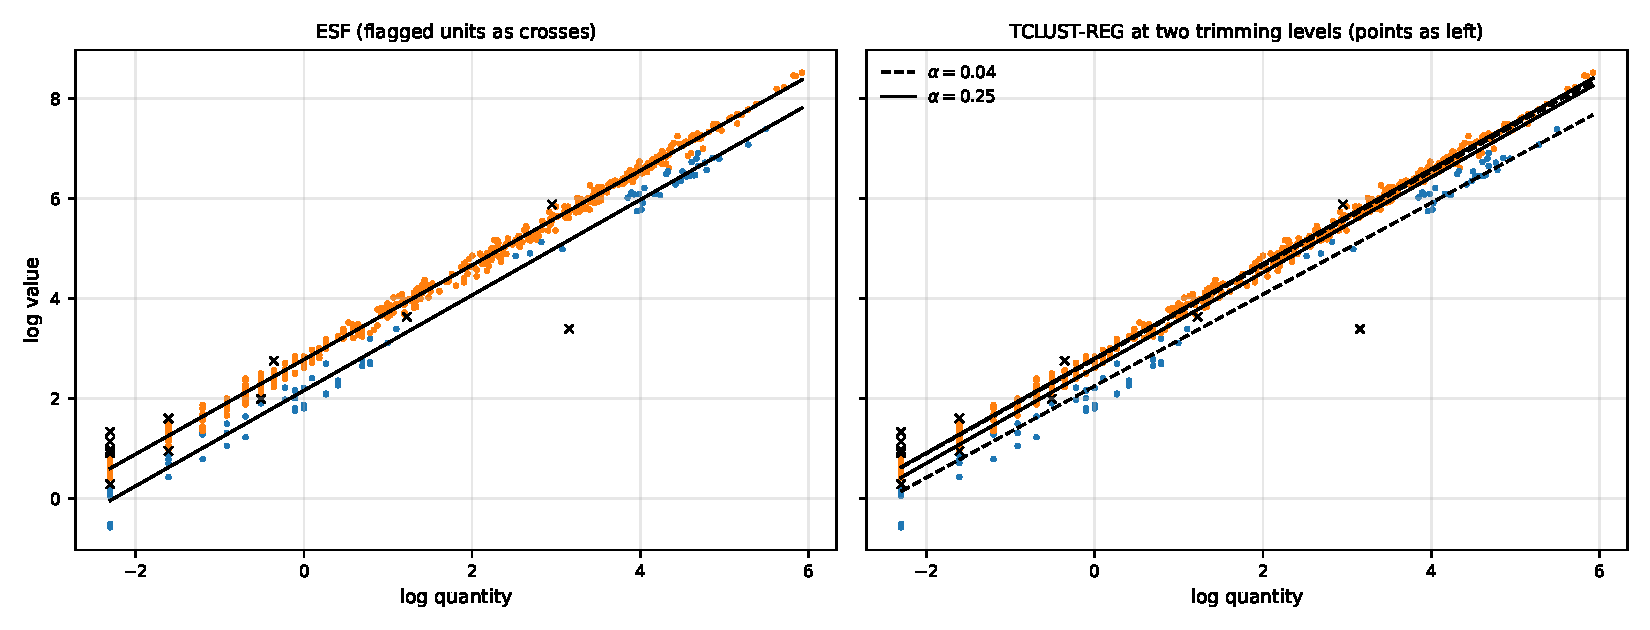
\includegraphics[width=0.9\textwidth]{figures/fishery.pdf}
\caption{Fishery data (Section~5.1 of the paper) on the logarithmic scale. Left: the two lines of ESF with the recovery
step (seed $0$), with its flagged flows as crosses and the other flows coloured by group.
Right: TCLUST-REG at trimming levels $0.04$ (dashed) and $0.25$ (solid), with the same
points.}
\label{fig:fishery}
\end{figure}

On the taxi data (Table~\ref{tab:taxi}), TLE at levels $0.10$ and $0.15$ and CTLE stopped with
an error on $18$, $19$ and $13$ of the $20$ samples; when they returned a fit, it was as
accurate as the best ($0.98$). The Laplace mixture fell below $0.7$ on $14$ samples, and least
squares on all.

\begin{table}[htbp]
\centering
\scriptsize
\caption{Fishery data (Section~5.1 of the paper), logarithmic scale, $K=2$: estimated
intercepts and slopes, median over random seeds or starts, with the range in brackets when it
exceeds $0.005$, and the trimmed or flagged fraction.}
\label{tab:fishery}
\resizebox{\textwidth}{!}{\begin{tabular}{lccc}
\toprule
Method & Group 1: intercept, slope & Group 2: intercept, slope & Trimmed or flagged \\
\midrule
ESF (20 seeds) & 2.16 [2.16, 2.58], 0.96 [0.95, 0.98] & 2.78 [2.78, 2.85], 0.94 & 0.03 [0.02, 0.12] \\
ESF alone (20 seeds) & 2.57 [2.56, 2.59], 0.98 [0.97, 0.98] & 2.85 [2.84, 2.86], 0.95 [0.94, 0.95] & 0.11 [0.10, 0.12] \\
TCLUST-REG, $\alpha=0.02$ (10 seeds) & 2.21, 0.93 & 2.78, 0.94 & 0.02 \\
TCLUST-REG, $\alpha=0.04$ (10 seeds) & 2.25, 0.92 & 2.78, 0.94 & 0.04 \\
TCLUST-REG, $\alpha=0.06$ (10 seeds) & 2.24, 0.92 & 2.78, 0.94 & 0.06 \\
TCLUST-REG, $\alpha=0.08$ (10 seeds) & 2.22 [2.22, 2.24], 0.92 & 2.78, 0.94 & 0.08 \\
TCLUST-REG, $\alpha=0.10$ (10 seeds) & 2.31 [1.91, 2.37], 0.94 [0.90, 0.99] & 2.77, 0.95 & 0.10 \\
TCLUST-REG, $\alpha=0.15$ (10 seeds) & 2.50 [1.81, 2.78], 0.94 [0.38, 0.95] & 2.79 [2.78, 2.84], 0.94 [0.79, 0.95] & 0.15 \\
TCLUST-REG, $\alpha=0.20$ (10 seeds) & 2.62 [2.56, 2.78], 0.95 [0.81, 1.07] & 2.78 [2.78, 2.80], 0.95 [0.81, 0.95] & 0.20 \\
TCLUST-REG, $\alpha=0.25$ (10 seeds) & 2.61 [2.55, 2.79], 0.96 [0.87, 1.01] & 2.79 [2.79, 2.87], 0.94 [0.84, 0.95] & 0.25 \\
TCLUST-REG, $\alpha=0.30$ (10 seeds) & 2.63 [2.55, 2.67], 0.95 [0.93, 1.03] & 2.80 [2.78, 2.82], 0.94 [0.94, 0.95] & 0.30 \\
CTLE (10 seeds) & 2.34, 0.94 & 2.79, 0.94 & 0.02 \\
Trimmed CWM, $\alpha=0.04$ (10 seeds) & 2.62 [2.28, 2.71], 0.89 [0.72, 0.97] & 2.80 [2.78, 2.80], 0.94 [0.82, 0.94] & 0.04 \\
Trimmed CWM, $\alpha=0.10$ (10 seeds) & 2.65 [2.56, 2.75], 0.96 [0.90, 1.00] & 2.78 [2.76, 2.85], 0.94 [0.83, 0.96] & 0.10 \\
Trimmed CWM, $\alpha=0.25$ (10 seeds) & 2.73 [2.57, 2.78], 0.96 [0.91, 1.00] & 2.79 [2.78, 2.84], 0.95 [0.94, 0.96] & 0.25 \\
\bottomrule
\end{tabular}}
\end{table}

\begin{table}[htbp]
\centering
\scriptsize
\caption{Taxi trips from JFK airport (Section~5.3 of the paper), $20$ random samples of
$2{,}000$ trips, $K=2$: mean and worst accuracy on the trips with rate codes 1 and 2, median
coefficient error against the flat fare ($70$, $0$, $0$) and a robust least-squares fit to all
metered trips of the month, mean flagged or trimmed fraction, and median time. A failed fit
counts as accuracy $0$. ``Reweighted'' is the rule of the paper, not that of
\citet{dotto2018reweighting}.}
\label{tab:taxi}
\resizebox{\textwidth}{!}{\begin{tabular}{lccccc}
\toprule
Method & Accuracy, mean & Accuracy, worst & Coefficient error & Flagged or trimmed & Time (s) \\
\midrule
ESF & 0.978 & 0.974 & 0.23 & 0.23 & 31 \\
ESF alone & 0.978 & 0.974 & 0.23 & 0.23 & 24 \\
TCLUST-REG (long search), $\alpha=0.25$, reweighted, then the recovery step & 0.979 & 0.975 & 0.10 & 0.14 & 86 \\
TCLUST-REG (long search), $\alpha=0.40$, reweighted, then the recovery step & 0.978 & 0.973 & 0.14 & 0.14 & 54 \\
TCLUST-REG (long search), $\alpha=0.25$, reweighted & 0.979 & 0.975 & 0.10 & 0.14 & 86 \\
TCLUST-REG (long search), $\alpha=0.40$, reweighted & 0.978 & 0.973 & 0.14 & 0.14 & 54 \\
TCLUST-REG, $\alpha=0.05$ & 0.972 & 0.959 & 0.98 & 0.05 & 7.30 \\
TCLUST-REG, $\alpha=0.10$ & 0.978 & 0.975 & 0.06 & 0.10 & 5.11 \\
TCLUST-REG, $\alpha=0.15$ & 0.978 & 0.975 & 0.09 & 0.15 & 4.35 \\
TCLUST-REG, $\alpha=0.25$ & 0.977 & 0.967 & 0.21 & 0.25 & 4.10 \\
TCLUST-REG, $\alpha=0.40$ & 0.975 & 0.965 & 0.48 & 0.40 & 3.02 \\
TCLUST-REG, $\alpha=0.25$, reweighted & 0.979 & 0.975 & 0.10 & 0.14 & 4.10 \\
TCLUST-REG, $\alpha=0.40$, reweighted & 0.978 & 0.970 & 0.13 & 0.14 & 3.02 \\
Trimmed CWM, $\alpha=0.05$ & 0.905 & 0.592 & 1.82 & 0.05 & 12 \\
Trimmed CWM, $\alpha=0.10$ & 0.978 & 0.975 & 0.06 & 0.10 & 12 \\
Trimmed CWM, $\alpha=0.15$ & 0.978 & 0.974 & 0.15 & 0.15 & 12 \\
Trimmed CWM, $\alpha=0.25$ & 0.978 & 0.970 & 0.20 & 0.25 & 11 \\
Trimmed CWM, $\alpha=0.40$ & 0.977 & 0.967 & 0.32 & 0.40 & 12 \\
TLE, $\alpha=0.05$ & 0.567 & 0.000 & 17.74 & 0.05 & 58 \\
TLE, $\alpha=0.10$ & 0.098 & 0.000 & 0.12 & 0.10 & 6.77 \\
TLE, $\alpha=0.15$ & 0.049 & 0.000 & 0.16 & 0.15 & 8.41 \\
TLE, $\alpha=0.25$ & 0.700 & 0.000 & 64.30 & 0.25 & 61 \\
TLE, $\alpha=0.40$ & 0.686 & 0.593 & 66.26 & 0.40 & 53 \\
CTLE & 0.342 & 0.000 & 0.24 & 0.09 & 80 \\
Bisquare mixture & 0.979 & 0.975 & 0.08 & 0.00 & 5.41 \\
Laplace mixture & 0.676 & 0.534 & 65.37 & 0.00 & 1136 \\
Contaminated normal mixture & 0.978 & 0.974 & 0.12 & 0.09 & 0.29 \\
Noise-component mixture & 0.978 & 0.974 & 0.23 & 0.08 & 0.04 \\
Least squares (50 starts) & 0.589 & 0.571 & 6.72 & -- & 0.07 \\
\bottomrule
\end{tabular}}
\end{table}

\begin{table}[htbp]
\centering
\scriptsize
\caption{Constants of ESF and of the recovery step (Section~2.5 of the paper), their values, the range examined, and the
largest change in a cell's mean accuracy over that range, up to $20\%$ of outliers unless
stated. For the loss cap the changes are relative to $c_{\mathrm b}=3$. S: table of this Supplement.}
\label{tab:constants}
\resizebox{\textwidth}{!}{%
\begin{tabular}{lllll}
\toprule
Constant & Value & Range examined & Change & Evidence \\
\midrule
\multicolumn{5}{l}{\emph{ESF (Algorithm~1 of the paper)}} \\
subsample size $m$ & $(d+1)/\pi_{\min}$ with room & up to $16$--$20$; $m=12$ everywhere & $0.02$; $0.035$ from $25\%$; $0.025$ (small groups); $0.07$ with four groups ($m=12$ for $16$) & S12, S15, S28, S39 \\
replicates $B$, stages $L$ & $100$, $10$ & $B=500$; $500$, $1000$ (fishery) & $-0.02$ to $+0.03$; $-0.07$ at $30\%$ & S29; Section~5.1 of the paper \\
cut-off $c$ & $2.5$ & $2$ to $3$ & $0.024$; $0.04$ at $30\%$ & S3 \\
loss cap $c_{\mathrm b}$ & $3$ & $3$ to $5$ & $0.13$ lost at $5$ (D5); $0.24$ gained with a group of $15\%$ & S13 \\
vote weight $\lambda$ & $3$ & $0$, $\infty$ & $0.05$ at $\lambda=0$ & S2 \\
covariate quantile & $0.975$ & $0.95$ to $0.99$ & $0.007$; $0.015$ at $30\%$; $0.21$ with leverage points & S3 \\
minimum group for screen & $\max(10,5p)$ & -- & -- & -- \\
\multicolumn{5}{l}{\emph{Recovery step (Algorithm~2 of the paper)}} \\
peak weight & $\tfrac12$ & $0.4$, $0.6$ & $0.015$ & S23 \\
window & $3c$ scales & $2c$, $4c$ & $0.03$ & S23 \\
minimum support & $\max\{2(d+1),0.03n\}$ & $0.02n$, $0.05n$ & $0.026$ & S23 \\
restriction factor & $12$ & $8$, $20$ & $0.016$ & S23 \\
margin & $\tfrac{d+1}{2}\log n$ & halved, doubled & $0.016$ & S23 \\
limit on flagged fraction & $n/3$ & $0.25n$, $0.40n$ & $0.20$ at $0.25n$ & S23 \\
noise range, random lines, applications & $1.1\,\mathrm{range}(y)$, $500$, $3$ & -- & -- & -- \\
\bottomrule
\end{tabular}}
\end{table}

\begin{table}[htbp]
\centering
\footnotesize
\caption{Criteria that count flagged or trimmed clean units (descriptive; Section~4.1 of the
paper), over the same $123$ cells as Table~2 of the paper: the adjusted Rand index on all units,
with the outliers as a class of their own and every flagged or trimmed unit labelled as an
outlier, and the misclassification rate of the clean units, counting a flagged clean unit as an
error (the labels matched to the true groups by the best permutation). Flags are those of the
reweighting rule ($c=2.5$), with the covariate screen for ESF and without it for TCLUST-REG.
Mean over cells of the cell means, and the worst cell. rw: the reweighting step; recovery:
followed by the recovery step.}
\label{tab:S45}
\resizebox{\textwidth}{!}{\begin{tabular}{lcccccccc}
\toprule
 & \multicolumn{4}{c}{$\varepsilon\le0.20$ (89 cells)} & \multicolumn{4}{c}{$\varepsilon\ge0.25$ (34 cells)} \\
\cmidrule(lr){2-5}\cmidrule(lr){6-9}
Method & ARI mean & ARI worst & Misc.\ mean & Misc.\ worst & ARI mean & ARI worst & Misc.\ mean & Misc.\ worst \\
\midrule
ESF & 0.719 & 0.54 & 0.102 & 0.29 & 0.660 & 0.01 & 0.183 & 0.48 \\
TCLUST-REG, $\alpha=0.25$, rw, recovery & 0.725 & 0.57 & 0.096 & 0.17 & 0.519 & 0.00 & 0.308 & 0.49 \\
TCLUST-REG, $\alpha=0.40$, rw, recovery & 0.715 & 0.56 & 0.104 & 0.19 & 0.714 & 0.01 & 0.138 & 0.48 \\
TCLUST-REG, $\alpha=0.25$, rw & 0.694 & 0.26 & 0.127 & 0.45 & 0.521 & 0.00 & 0.306 & 0.49 \\
TCLUST-REG, $\alpha=0.40$, rw & 0.624 & 0.24 & 0.201 & 0.52 & 0.720 & 0.02 & 0.133 & 0.47 \\
\bottomrule
\end{tabular}}
\end{table}

\begin{table}[htbp]
\centering
\footnotesize
\caption{The recovery step after the trimmed cluster-weighted model (descriptive;
Section~4.6 of the paper): mean over cells of the mean accuracy on clean units, the number of
cells with a mean below $0.85$, and the worst cell, over the same $123$ cells as Table~2 of the
paper. The model is fitted by RobMixReg at levels $0.25$ and $0.40$ ($50$ starts), then
reweighted by our rule (rw) and followed by the recovery step.}
\label{tab:S46}
\resizebox{\textwidth}{!}{\begin{tabular}{lcccccc}
\toprule
 & \multicolumn{3}{c}{$\varepsilon\le0.20$ (89 cells)} & \multicolumn{3}{c}{$\varepsilon\ge0.25$ (34 cells)} \\
\cmidrule(lr){2-4}\cmidrule(lr){5-7}
Method & Mean & Below $0.85$ & Worst & Mean & Below $0.85$ & Worst \\
\midrule
Trimmed CWM, $\alpha=0.25$, alone & 0.786 & 47 & 0.57 & 0.677 & 32 & 0.53 \\
Trimmed CWM, $\alpha=0.25$, rw & 0.804 & 39 & 0.56 & 0.682 & 32 & 0.53 \\
Trimmed CWM, $\alpha=0.25$, rw, recovery & 0.882 & 12 & 0.66 & 0.679 & 31 & 0.53 \\
Trimmed CWM, $\alpha=0.40$, alone & 0.716 & 77 & 0.56 & 0.759 & 28 & 0.58 \\
Trimmed CWM, $\alpha=0.40$, rw & 0.745 & 66 & 0.54 & 0.786 & 24 & 0.61 \\
Trimmed CWM, $\alpha=0.40$, rw, recovery & 0.871 & 20 & 0.64 & 0.785 & 24 & 0.62 \\
\bottomrule
\end{tabular}}
\end{table}

\begin{table}[htbp]
\centering
\scriptsize
\caption{The five analysis plans (Section~4.1 of the paper): what each fixed before the data it concerns were analysed
(Plans~1 and~2) or generated (Plans~3 to~5), and the data it concerns. The third part of the
study ($2{,}300$ data sets) is descriptive and had no plan.}
\label{tab:plans}
\begin{tabular}{@{}lp{6.5cm}p{5.0cm}@{}}
\toprule
Plan & What it fixed & Data it concerns \\
\midrule
1 & ESF alone against the best competitor chosen after the run in each cell: mean paired
difference not below $-0.03$, upper $95\%$ bound not below $-0.02$; every fixed-level
competitor to fall $0.05$ below ESF alone somewhere & First part: D1 to D8,
$\varepsilon\in\{0,0.05,0.10,0.20,0.30\}$, $50$ data sets per cell, $2{,}000$; the comparison
concerns $\varepsilon\le0.20$ \\
2 & Whether TCLUST-REG at level $0.25$ with reweighting fails above its level while ESF alone
does not (gap of $0.05$, interval excluding zero, in some design without high-leverage points)
& Second part: $\varepsilon\in\{0.25,0.30,0.35\}$, new data, $100$ per cell, $2{,}400$ \\
3 & The recovery step, code frozen: gain of at least $0.05$ in the small-group cells, no loss
above $0.01$ at $\varepsilon\le0.20$, the comparison of Plan~1 for ESF with the step & The
stored fits of ESF alone on the $6{,}400$ data sets of the first three parts \\
4 & The same confirmation on fresh data & $600$ new data sets in four small-group designs \\
5 & The comparison of Plan~1 in three designs outside the Gaussian family & $450$ new data sets \\
\bottomrule
\end{tabular}
\end{table}

\begin{table}[htbp]
\centering
\footnotesize
\caption{Sensitivity of the recovery step to its noise range (descriptive; Section~4.6 of the
paper): the range $R$, $1.1$ times the range of the response, multiplied by $2$ and $5$, as if
the most extreme unit lay two or five times farther out, and replaced by two ranges tied to the
fitted scales ($20$ median group scales; the range of the unflagged units plus $10$ median
scales); mean over cells of the mean accuracy
on clean units, the number of cells with a mean below $0.85$, and the worst cell, over the same
$123$ cells as Table~2 of the paper. Fits and seeds as in the study.}
\label{tab:S48}
\resizebox{\textwidth}{!}{\begin{tabular}{lcccccc}
\toprule
 & \multicolumn{3}{c}{$\varepsilon\le0.20$ (89 cells)} & \multicolumn{3}{c}{$\varepsilon\ge0.25$ (34 cells)} \\
\cmidrule(lr){2-4}\cmidrule(lr){5-7}
Method & Mean & Below $0.85$ & Worst & Mean & Below $0.85$ & Worst \\
\midrule
ESF, range $R$ as in the paper & 0.914 & 2 & 0.78 & 0.820 & 13 & 0.53 \\
ESF, range $2R$ & 0.912 & 2 & 0.69 & 0.812 & 15 & 0.53 \\
ESF, range $5R$ & 0.910 & 3 & 0.68 & 0.799 & 16 & 0.53 \\
ESF, range $20$ median scales & 0.891 & 12 & 0.62 & 0.819 & 13 & 0.53 \\
ESF, unflagged range plus $10$ median scales & 0.903 & 9 & 0.70 & 0.817 & 13 & 0.53 \\
TCLUST-REG $0.40$, rw, recovery, range $R$ & 0.909 & 4 & 0.81 & 0.863 & 8 & 0.53 \\
TCLUST-REG $0.40$, rw, recovery, range $2R$ & 0.908 & 5 & 0.81 & 0.846 & 10 & 0.54 \\
TCLUST-REG $0.40$, rw, recovery, range $5R$ & 0.906 & 7 & 0.75 & 0.830 & 12 & 0.54 \\
TCLUST-REG $0.40$, rw, recovery, $20$ median scales & 0.883 & 15 & 0.61 & 0.859 & 9 & 0.54 \\
TCLUST-REG $0.40$, rw, recovery, unflagged range plus $10$ scales & 0.899 & 10 & 0.73 & 0.853 & 9 & 0.54 \\
\bottomrule
\end{tabular}}
\end{table}

\begin{table}[htbp]
\centering
\footnotesize
\caption{TCLUST-REG's own assignment against the criterion of the paper (descriptive;
Section~4.1 of the paper): mean accuracy on clean units of the long-search fits at levels $0.25$
and $0.40$ (without reweighting) when every clean unit takes the label of its nearest fitted line,
as in the paper, and when it takes the label that TCLUST-REG assigns (\texttt{out.idx}), trimmed
clean units then taking that of their nearest line; and the fraction of clean units trimmed.
Same fits and data sets as the study.}
\label{tab:S49}
\resizebox{\textwidth}{!}{\begin{tabular}{llcccccc}
\toprule
 & & \multicolumn{3}{c}{$\alpha=0.25$} & \multicolumn{3}{c}{$\alpha=0.40$} \\
\cmidrule(lr){3-5}\cmidrule(lr){6-8}
Design & $\varepsilon$ & Nearest line & Own assignment & Clean trimmed & Nearest line & Own assignment & Clean trimmed \\
\midrule
D2 & 0.00 & 0.876 & 0.868 & 0.250 & 0.794 & 0.792 & 0.400 \\
D2 & 0.05 & 0.883 & 0.874 & 0.213 & 0.830 & 0.829 & 0.371 \\
D2 & 0.10 & 0.891 & 0.878 & 0.165 & 0.841 & 0.837 & 0.332 \\
D2 & 0.20 & 0.883 & 0.861 & 0.065 & 0.840 & 0.832 & 0.251 \\
D4 & 0.00 & 0.911 & 0.917 & 0.250 & 0.908 & 0.916 & 0.400 \\
D4 & 0.05 & 0.908 & 0.914 & 0.210 & 0.905 & 0.911 & 0.368 \\
D4 & 0.10 & 0.909 & 0.918 & 0.167 & 0.907 & 0.912 & 0.333 \\
D4 & 0.20 & 0.907 & 0.925 & 0.066 & 0.905 & 0.911 & 0.252 \\
D2 & 0.25 & 0.756 & 0.735 & 0.018 & 0.857 & 0.847 & 0.195 \\
D2 & 0.30 & 0.618 & 0.604 & 0.005 & 0.859 & 0.838 & 0.141 \\
D2 & 0.35 & 0.507 & 0.497 & 0.002 & 0.834 & 0.801 & 0.076 \\
D4 & 0.25 & 0.875 & 0.896 & 0.013 & 0.911 & 0.917 & 0.199 \\
D4 & 0.30 & 0.617 & 0.621 & 0.004 & 0.910 & 0.918 & 0.140 \\
D4 & 0.35 & 0.530 & 0.531 & 0.003 & 0.911 & 0.926 & 0.072 \\
$K=4$ & 0.00 & 0.925 & 0.929 & 0.250 & 0.792 & 0.809 & 0.400 \\
$K=4$ & 0.10 & 0.932 & 0.932 & 0.168 & 0.794 & 0.809 & 0.334 \\
$K=4$ & 0.20 & 0.896 & 0.884 & 0.068 & 0.795 & 0.805 & 0.256 \\
$K=4$ & 0.30 & 0.748 & 0.749 & 0.004 & 0.758 & 0.756 & 0.150 \\
\bottomrule
\end{tabular}}
\end{table}

\begin{table}[htbp]
\centering
\footnotesize
\caption{The eleven cells that decide the comparison up to $20\%$ of outliers, with $200$ data
sets each: the $50$ of the study and $150$ further ones from the same generators (descriptive;
Section~4.2 of the paper). Mean accuracy on clean units of ESF with its standard error, and, for
TCLUST-REG with the long search, reweighting and the recovery step at level $0.25$, at level
$0.30$ and at level $0.25$ with equal weights, the mean and the paired difference ESF minus that
pipeline with its standard error.}
\label{tab:S50}
\resizebox{\textwidth}{!}{\begin{tabular}{llcccccccc}
\toprule
Design & $\varepsilon$ & $n_{\mathrm{rep}}$ & ESF & \multicolumn{2}{c}{$0.25$} & \multicolumn{2}{c}{$0.30$} & \multicolumn{2}{c}{$0.25$, equal weights} \\
\cmidrule(lr){5-6}\cmidrule(lr){7-8}\cmidrule(lr){9-10}
 & & & mean (s.e.) & mean & ESF $-$ (s.e.) & mean & ESF $-$ (s.e.) & mean & ESF $-$ (s.e.) \\
\midrule
D2 & 0.00 & 200 & 0.905 (0.001) & 0.889 & +0.016 (0.003) & 0.876 & +0.029 (0.005) & 0.897 & +0.008 (0.002) \\
D2 & 0.05 & 200 & 0.903 (0.002) & 0.893 & +0.010 (0.003) & 0.886 & +0.017 (0.004) & 0.899 & +0.004 (0.002) \\
D2 & 0.10 & 200 & 0.899 (0.003) & 0.899 & -0.000 (0.003) & 0.889 & +0.009 (0.004) & 0.900 & -0.002 (0.003) \\
D2 & 0.20 & 200 & 0.904 (0.003) & 0.891 & +0.012 (0.004) & 0.901 & +0.003 (0.003) & 0.906 & -0.003 (0.002) \\
$K=4$ & 0.00 & 200 & 0.961 (0.002) & 0.929 & +0.032 (0.006) & 0.901 & +0.060 (0.007) & 0.963 & -0.002 (0.002) \\
$K=4$ & 0.10 & 200 & 0.959 (0.002) & 0.923 & +0.036 (0.006) & 0.898 & +0.061 (0.007) & 0.962 & -0.003 (0.002) \\
$K=4$ & 0.20 & 200 & 0.945 (0.005) & 0.901 & +0.044 (0.008) & 0.888 & +0.058 (0.008) & 0.955 & -0.010 (0.005) \\
80/20 & 0.20 & 200 & 0.883 (0.007) & 0.910 & -0.027 (0.007) & 0.909 & -0.026 (0.007) & 0.909 & -0.026 (0.007) \\
clustered & 0.20 & 200 & 0.810 (0.012) & 0.904 & -0.094 (0.012) & 0.909 & -0.100 (0.012) & 0.910 & -0.100 (0.012) \\
80/20, $p=3$ & 0.20 & 200 & 0.850 (0.009) & 0.907 & -0.057 (0.009) & 0.896 & -0.046 (0.010) & 0.900 & -0.050 (0.009) \\
85/15, parallel & 0.20 & 200 & 0.880 (0.013) & 0.967 & -0.088 (0.011) & 0.962 & -0.083 (0.011) & 0.964 & -0.085 (0.011) \\
\bottomrule
\end{tabular}}
\end{table}
